% Created by tikzDevice version 0.12.6 on 2024-03-12 19:53:25
% !TEX encoding = UTF-8 Unicode
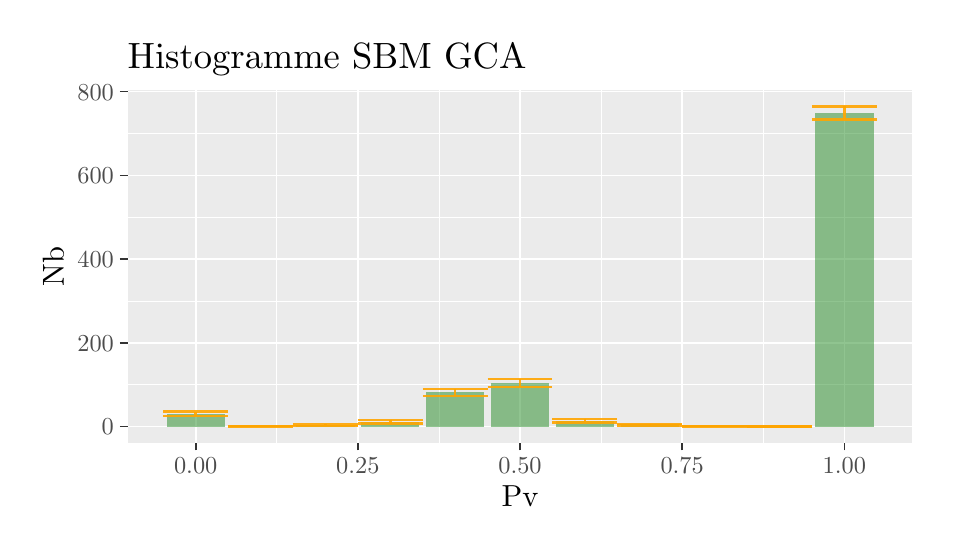
\begin{tikzpicture}[x=1pt,y=1pt]
\definecolor{fillColor}{RGB}{255,255,255}
\path[use as bounding box,fill=fillColor,fill opacity=0.00] (0,0) rectangle (325.21,180.67);
\begin{scope}
\path[clip] (  0.00,  0.00) rectangle (325.21,180.67);
\definecolor{drawColor}{RGB}{255,255,255}
\definecolor{fillColor}{RGB}{255,255,255}

\path[draw=drawColor,line width= 0.6pt,line join=round,line cap=round,fill=fillColor] (  0.00,  0.00) rectangle (325.21,180.68);
\end{scope}
\begin{scope}
\path[clip] ( 36.11, 30.69) rectangle (319.71,158.02);
\definecolor{fillColor}{gray}{0.92}

\path[fill=fillColor] ( 36.11, 30.69) rectangle (319.71,158.02);
\definecolor{drawColor}{RGB}{255,255,255}

\path[draw=drawColor,line width= 0.3pt,line join=round] ( 36.11, 51.65) --
	(319.71, 51.65);

\path[draw=drawColor,line width= 0.3pt,line join=round] ( 36.11, 81.91) --
	(319.71, 81.91);

\path[draw=drawColor,line width= 0.3pt,line join=round] ( 36.11,112.17) --
	(319.71,112.17);

\path[draw=drawColor,line width= 0.3pt,line join=round] ( 36.11,142.43) --
	(319.71,142.43);

\path[draw=drawColor,line width= 0.3pt,line join=round] ( 90.02, 30.69) --
	( 90.02,158.02);

\path[draw=drawColor,line width= 0.3pt,line join=round] (148.62, 30.69) --
	(148.62,158.02);

\path[draw=drawColor,line width= 0.3pt,line join=round] (207.21, 30.69) --
	(207.21,158.02);

\path[draw=drawColor,line width= 0.3pt,line join=round] (265.81, 30.69) --
	(265.81,158.02);

\path[draw=drawColor,line width= 0.6pt,line join=round] ( 36.11, 36.52) --
	(319.71, 36.52);

\path[draw=drawColor,line width= 0.6pt,line join=round] ( 36.11, 66.78) --
	(319.71, 66.78);

\path[draw=drawColor,line width= 0.6pt,line join=round] ( 36.11, 97.04) --
	(319.71, 97.04);

\path[draw=drawColor,line width= 0.6pt,line join=round] ( 36.11,127.30) --
	(319.71,127.30);

\path[draw=drawColor,line width= 0.6pt,line join=round] ( 36.11,157.56) --
	(319.71,157.56);

\path[draw=drawColor,line width= 0.6pt,line join=round] ( 60.72, 30.69) --
	( 60.72,158.02);

\path[draw=drawColor,line width= 0.6pt,line join=round] (119.32, 30.69) --
	(119.32,158.02);

\path[draw=drawColor,line width= 0.6pt,line join=round] (177.91, 30.69) --
	(177.91,158.02);

\path[draw=drawColor,line width= 0.6pt,line join=round] (236.51, 30.69) --
	(236.51,158.02);

\path[draw=drawColor,line width= 0.6pt,line join=round] (295.10, 30.69) --
	(295.10,158.02);
\definecolor{fillColor}{RGB}{34,139,34}

\path[fill=fillColor,fill opacity=0.50] ( 50.17, 36.52) rectangle ( 71.27, 41.12);

\path[fill=fillColor,fill opacity=0.50] ( 73.61, 36.52) rectangle ( 94.71, 36.57);

\path[fill=fillColor,fill opacity=0.50] ( 97.05, 36.52) rectangle (118.15, 37.02);

\path[fill=fillColor,fill opacity=0.50] (120.49, 36.52) rectangle (141.58, 38.23);

\path[fill=fillColor,fill opacity=0.50] (143.93, 36.52) rectangle (165.02, 48.84);

\path[fill=fillColor,fill opacity=0.50] (167.37, 36.52) rectangle (188.46, 52.34);

\path[fill=fillColor,fill opacity=0.50] (190.80, 36.52) rectangle (211.90, 38.67);

\path[fill=fillColor,fill opacity=0.50] (214.24, 36.52) rectangle (235.34, 37.18);

\path[fill=fillColor,fill opacity=0.50] (237.68, 36.52) rectangle (258.78, 36.60);

\path[fill=fillColor,fill opacity=0.50] (261.12, 36.52) rectangle (282.21, 36.52);

\path[fill=fillColor,fill opacity=0.50] (284.56, 36.52) rectangle (305.65,149.90);
\definecolor{drawColor}{RGB}{255,165,0}

\path[draw=drawColor,draw opacity=0.90,line width= 0.9pt,line join=round] ( 49.00, 41.91) --
	( 72.44, 41.91);

\path[draw=drawColor,draw opacity=0.90,line width= 0.9pt,line join=round] ( 60.72, 41.91) --
	( 60.72, 40.33);

\path[draw=drawColor,draw opacity=0.90,line width= 0.9pt,line join=round] ( 49.00, 40.33) --
	( 72.44, 40.33);

\path[draw=drawColor,draw opacity=0.90,line width= 0.9pt,line join=round] ( 72.44, 36.67) --
	( 95.88, 36.67);

\path[draw=drawColor,draw opacity=0.90,line width= 0.9pt,line join=round] ( 84.16, 36.67) --
	( 84.16, 36.47);

\path[draw=drawColor,draw opacity=0.90,line width= 0.9pt,line join=round] ( 72.44, 36.47) --
	( 95.88, 36.47);

\path[draw=drawColor,draw opacity=0.90,line width= 0.9pt,line join=round] ( 95.88, 37.30) --
	(119.32, 37.30);

\path[draw=drawColor,draw opacity=0.90,line width= 0.9pt,line join=round] (107.60, 37.30) --
	(107.60, 36.74);

\path[draw=drawColor,draw opacity=0.90,line width= 0.9pt,line join=round] ( 95.88, 36.74) --
	(119.32, 36.74);

\path[draw=drawColor,draw opacity=0.90,line width= 0.9pt,line join=round] (119.32, 38.91) --
	(142.76, 38.91);

\path[draw=drawColor,draw opacity=0.90,line width= 0.9pt,line join=round] (131.04, 38.91) --
	(131.04, 37.55);

\path[draw=drawColor,draw opacity=0.90,line width= 0.9pt,line join=round] (119.32, 37.55) --
	(142.76, 37.55);

\path[draw=drawColor,draw opacity=0.90,line width= 0.9pt,line join=round] (142.76, 50.04) --
	(166.19, 50.04);

\path[draw=drawColor,draw opacity=0.90,line width= 0.9pt,line join=round] (154.47, 50.04) --
	(154.47, 47.64);

\path[draw=drawColor,draw opacity=0.90,line width= 0.9pt,line join=round] (142.76, 47.64) --
	(166.19, 47.64);

\path[draw=drawColor,draw opacity=0.90,line width= 0.9pt,line join=round] (166.19, 53.78) --
	(189.63, 53.78);

\path[draw=drawColor,draw opacity=0.90,line width= 0.9pt,line join=round] (177.91, 53.78) --
	(177.91, 50.90);

\path[draw=drawColor,draw opacity=0.90,line width= 0.9pt,line join=round] (166.19, 50.90) --
	(189.63, 50.90);

\path[draw=drawColor,draw opacity=0.90,line width= 0.9pt,line join=round] (189.63, 39.29) --
	(213.07, 39.29);

\path[draw=drawColor,draw opacity=0.90,line width= 0.9pt,line join=round] (201.35, 39.29) --
	(201.35, 38.05);

\path[draw=drawColor,draw opacity=0.90,line width= 0.9pt,line join=round] (189.63, 38.05) --
	(213.07, 38.05);

\path[draw=drawColor,draw opacity=0.90,line width= 0.9pt,line join=round] (213.07, 37.52) --
	(236.51, 37.52);

\path[draw=drawColor,draw opacity=0.90,line width= 0.9pt,line join=round] (224.79, 37.52) --
	(224.79, 36.84);

\path[draw=drawColor,draw opacity=0.90,line width= 0.9pt,line join=round] (213.07, 36.84) --
	(236.51, 36.84);

\path[draw=drawColor,draw opacity=0.90,line width= 0.9pt,line join=round] (236.51, 36.71) --
	(259.95, 36.71);

\path[draw=drawColor,draw opacity=0.90,line width= 0.9pt,line join=round] (248.23, 36.71) --
	(248.23, 36.49);

\path[draw=drawColor,draw opacity=0.90,line width= 0.9pt,line join=round] (236.51, 36.49) --
	(259.95, 36.49);

\path[draw=drawColor,draw opacity=0.90,line width= 0.9pt,line join=round] (259.95, 36.55) --
	(283.39, 36.55);

\path[draw=drawColor,draw opacity=0.90,line width= 0.9pt,line join=round] (271.67, 36.55) --
	(271.67, 36.50);

\path[draw=drawColor,draw opacity=0.90,line width= 0.9pt,line join=round] (259.95, 36.50) --
	(283.39, 36.50);

\path[draw=drawColor,draw opacity=0.90,line width= 0.9pt,line join=round] (283.39,152.23) --
	(306.82,152.23);

\path[draw=drawColor,draw opacity=0.90,line width= 0.9pt,line join=round] (295.10,152.23) --
	(295.10,147.56);

\path[draw=drawColor,draw opacity=0.90,line width= 0.9pt,line join=round] (283.39,147.56) --
	(306.82,147.56);
\end{scope}
\begin{scope}
\path[clip] (  0.00,  0.00) rectangle (325.21,180.67);
\definecolor{drawColor}{gray}{0.30}

\node[text=drawColor,anchor=base east,inner sep=0pt, outer sep=0pt, scale=  0.88] at ( 31.16, 33.49) {0};

\node[text=drawColor,anchor=base east,inner sep=0pt, outer sep=0pt, scale=  0.88] at ( 31.16, 63.75) {200};

\node[text=drawColor,anchor=base east,inner sep=0pt, outer sep=0pt, scale=  0.88] at ( 31.16, 94.01) {400};

\node[text=drawColor,anchor=base east,inner sep=0pt, outer sep=0pt, scale=  0.88] at ( 31.16,124.27) {600};

\node[text=drawColor,anchor=base east,inner sep=0pt, outer sep=0pt, scale=  0.88] at ( 31.16,154.53) {800};
\end{scope}
\begin{scope}
\path[clip] (  0.00,  0.00) rectangle (325.21,180.67);
\definecolor{drawColor}{gray}{0.20}

\path[draw=drawColor,line width= 0.6pt,line join=round] ( 33.36, 36.52) --
	( 36.11, 36.52);

\path[draw=drawColor,line width= 0.6pt,line join=round] ( 33.36, 66.78) --
	( 36.11, 66.78);

\path[draw=drawColor,line width= 0.6pt,line join=round] ( 33.36, 97.04) --
	( 36.11, 97.04);

\path[draw=drawColor,line width= 0.6pt,line join=round] ( 33.36,127.30) --
	( 36.11,127.30);

\path[draw=drawColor,line width= 0.6pt,line join=round] ( 33.36,157.56) --
	( 36.11,157.56);
\end{scope}
\begin{scope}
\path[clip] (  0.00,  0.00) rectangle (325.21,180.67);
\definecolor{drawColor}{gray}{0.20}

\path[draw=drawColor,line width= 0.6pt,line join=round] ( 60.72, 27.94) --
	( 60.72, 30.69);

\path[draw=drawColor,line width= 0.6pt,line join=round] (119.32, 27.94) --
	(119.32, 30.69);

\path[draw=drawColor,line width= 0.6pt,line join=round] (177.91, 27.94) --
	(177.91, 30.69);

\path[draw=drawColor,line width= 0.6pt,line join=round] (236.51, 27.94) --
	(236.51, 30.69);

\path[draw=drawColor,line width= 0.6pt,line join=round] (295.10, 27.94) --
	(295.10, 30.69);
\end{scope}
\begin{scope}
\path[clip] (  0.00,  0.00) rectangle (325.21,180.67);
\definecolor{drawColor}{gray}{0.30}

\node[text=drawColor,anchor=base,inner sep=0pt, outer sep=0pt, scale=  0.88] at ( 60.72, 19.68) {0.00};

\node[text=drawColor,anchor=base,inner sep=0pt, outer sep=0pt, scale=  0.88] at (119.32, 19.68) {0.25};

\node[text=drawColor,anchor=base,inner sep=0pt, outer sep=0pt, scale=  0.88] at (177.91, 19.68) {0.50};

\node[text=drawColor,anchor=base,inner sep=0pt, outer sep=0pt, scale=  0.88] at (236.51, 19.68) {0.75};

\node[text=drawColor,anchor=base,inner sep=0pt, outer sep=0pt, scale=  0.88] at (295.10, 19.68) {1.00};
\end{scope}
\begin{scope}
\path[clip] (  0.00,  0.00) rectangle (325.21,180.67);
\definecolor{drawColor}{RGB}{0,0,0}

\node[text=drawColor,anchor=base,inner sep=0pt, outer sep=0pt, scale=  1.10] at (177.91,  7.64) {Pv};
\end{scope}
\begin{scope}
\path[clip] (  0.00,  0.00) rectangle (325.21,180.67);
\definecolor{drawColor}{RGB}{0,0,0}

\node[text=drawColor,rotate= 90.00,anchor=base,inner sep=0pt, outer sep=0pt, scale=  1.10] at ( 13.08, 94.35) {Nb};
\end{scope}
\begin{scope}
\path[clip] (  0.00,  0.00) rectangle (325.21,180.67);
\definecolor{drawColor}{RGB}{0,0,0}

\node[text=drawColor,anchor=base west,inner sep=0pt, outer sep=0pt, scale=  1.32] at ( 36.11,166.08) {Histogramme SBM GCA};
\end{scope}
\end{tikzpicture}
